\documentclass{ximera}

\outcome{Identify an improper integral.}
\outcome{Determine if an improper integral converges or diverges.}
\outcome{Compute integrals over infinite intervals.}
\outcome{Compute integrals of functions with vertical asymptotes.}
\author{Jason Miller and Jim Talamo}
\newcommand{\RR}{\mathbb R}
\renewcommand{\d}{\,d}
\newcommand{\dd}[2][]{\frac{d #1}{d #2}}
\renewcommand{\l}{\ell}
\newcommand{\ddx}{\frac{d}{dx}}
\newcommand{\dfn}{\textbf}
\newcommand{\eval}[1]{\bigg[ #1 \bigg]}


\title[Dig-In:]{Improper Integrals}

\begin{document}
\begin{abstract}
  We can use limits to integrate functions on unbounded domains or functions with unbounded range.
\end{abstract}
\maketitle


Recall that we introduced the definite integral

\[
\int_a^b f(x) \d x,
\]

as a limit of Riemann sums.  This limit need not always exist, as it depends on the properties of the
function $f$ on the given interval $[a, b]$.  When the function $f$ is \emph{continuous} on $[a,b]$, this 
definite integral represents the net between the graph of $y=f(x)$ and the $x$-axis on $a \leq x \leq b$

\begin{image}
\begin{tikzpicture}

\begin{axis}
	[
	domain=0:6, ymax=1.75,xmax=6, ymin=0, xmin=0,
	axis lines=center, xlabel=$x$, ylabel=$y$,
	xtick={1.5,4.5},
	xticklabels={$a$,$b$},
	ymajorticks=false,
	every axis y label/.style={at=(current axis.above origin),anchor=south},
	every axis x label/.style={at=(current axis.right of origin),anchor=west},
	axis on top,
	typeset ticklabels with strut,
	]

	\addplot [draw=penColor,very thick, smooth] {.4*sin(deg(x)) + 1};
	
	\addplot [name path=A,domain=1.5:4.5,draw=none] {.4*sin(deg(x)) + 1};   
	\addplot [name path=B,domain=1.5:4.5,draw=none] {0};
	\addplot [fillp] fill between[of=A and B];
	
	\draw[penColor,thick] (1.5,0) -- (1.5,{.4*sin(deg(1.5)) + 1});
	\draw[penColor,thick] (4.5,0) -- (4.5,{.4*sin(deg(4.5)) + 1});
	
	\node at (axis cs:3,1.5) [penColor] {$y=f(x)$};
\end{axis}

\end{tikzpicture}
\end{image}


and the Fundamental Theorem of Calculus comes to the rescue and assures us that 

\begin{image}
  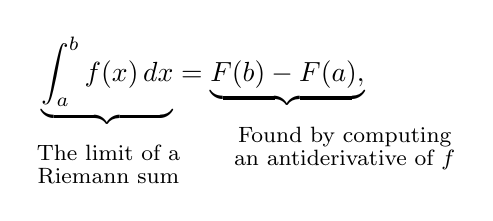
\begin{tikzpicture}
        \node at (0,0) {
          $\underbrace{\int_a^b f(x) \d x} = \underbrace{F(b)-F(a),}$};
         \node at (-1.2,-.9)   {\footnotesize{The limit of a}};
        \node at (-1.2,-1.2)  {\footnotesize{Riemann sum}};
        
       \node at (1.8,-.7){\footnotesize{Found by computing }};
        \node at (1.8,-1) {\footnotesize{an antiderivative of $f$}};    
        
        
      \end{tikzpicture}
  \end{image}

where $F(x)$ is an antiderivative of $f(x)$.

Note that while explicitly computing the limit of Riemann sums is an arduous task, the Fundamental Theorem of Calculus allows us to use antiderivatives to accomplish the same task.  However, note that there are two requirements that the function must satisfy before we can apply the Fundamental Theorem.

\begin{itemize}
\item The interval over which we integrated, $[a,b]$, must be a closed interval of finite length, and
\item The function $f$ must be bounded on $[a,b]$.
\end{itemize}


\begin{remark}
Recall that in order for a function defined on $[a, b]$ to be bounded on $[a,b]$, there must be some real number $M>0$ such that 
\[
|f(x)| \leq M \text{ for all } x \text{ in } [a, b]
\]

This says that the outputs of $f$ are trapped between the horizontal lines $y=-M$ and $y=M$; the output values cannot 
become arbitrarily large in either the positive or negative sense on $[a,b]$. 
\end{remark}


It turns out that there are many instances where these limitations are a problem.  For instance, there are applications in statistics, physics, and engineering where we need to integrate over unbounded regions or we need to integrate unbounded functions.  In this section, we will generalize the notion of the integral in such a way to overcome each of the restrictions above.



\begin{definition}
  An integral $\int_a^b f(x) \d x $
  is called an \dfn{improper integral} if one of, or both, of the conditions hold:
  \begin{itemize}
  \item The interval of integration is infinite.
  \item The function $f$ is unbounded on the interval of integration.
  \end{itemize}
\end{definition}

\begin{question}
  Which of the following integrals are improper according to the previous definition?
  \begin{selectAll}
    \choice{$\int_{-1}^{100} \frac{1}{1+x^2} \d x$}
    \choice[correct]{$\int_{1}^{\infty}\frac{1}{1+x^2}\d x$}
    \choice[correct]{$\int_0^1 \ln(x) \d x$}
    \choice{$\int_0^1 \frac{\sin(x)}{x} \d x$}
    \choice[correct]{$\int_{-\infty}^{\infty} \sin(x) \d x$}
    \choice[correct]{$\int_{0}^{\pi} \tan(x) \d x$}
  \end{selectAll}

\begin{feedback}
\begin{itemize}
\item Note that $\frac{1}{1+x^2}$ is continuous everywhere, so it is bounded on any finite interval. 
\item $\lim_{x \to 0^+} \ln(x) = -\infty$, so $\ln(x)$ is unbounded on $[0,1]$.
\item $\lim_{x \to 0^+} \frac{\sin(x)}{x} = 1$, so even though $\frac{\sin(x)}{x}$ is not continuous at $x=0$, it is bounded on $[0,1]$.  Hence $\int_0^1 \frac{\sin(x)}{x} \d x$ is proper.
\item $\tan(x)$ has a vertical asymptote at $x=\frac{\pi}{2}$, so it is unbounded on $[0,\pi]$.
\end{itemize}
\end{feedback}
\end{question}





\section{Unbounded intervals}


Consider the expression
\[ 
\int_{a}^{\infty} f(x) \d x
\]
What does this expression mean?  Let's consider a particular example and see if we can make sense of it.

\begin{example}
Evaluate the improper integral
\[ 
\int_{1}^{\infty} \frac{1}{x} \d x
\]
\begin{explanation}

We interpret definite integrals as giving us the net area underneath the graph of the function over the given interval. If we used this interpretation here, this notation should mean that we want to find the area under $\frac{1}{x}$ from $1$ to $\infty$.  This idea needs to be more precisely defined.  Let's consider the definite integral
\[
\int_{1}^{b} \frac{1}{x} \d x=\eval{\ln|x|}_{1}^{b}=\ln(b)
\]

where $b \geq 1$ is some fixed number. 

\begin{image}
  \begin{tikzpicture}
  \begin{axis}[
      xmin=0, xmax=4,ymin=-.3,ymax=1.1,domain=.001:1,
      axis lines = center, xlabel=$x$, ylabel=$y$,
      xtick={1,2,3},
      ytick={0.5,1},
      every axis y label/.style={at=(current axis.above origin),anchor=south},
      every axis x label/.style={at=(current axis.right of origin),anchor=west},
      axis on top,
%      width=6in,
%      height=3in,
    ] 
    \addplot [draw=none, fill=fillp,domain=1:3.75 ] {1/x} \closedcycle;
    \addplot [penColor,very thick, smooth,domain=.5:10,samples=100] {1/x};
    \addplot [penColor, smooth,domain=0:.267] (3.75,x); 
    \addplot [penColor, smooth,domain=0:1] (1,x);
    \node at (axis cs:3.75,-.075) {$N$};
    \node at (axis cs:2,1) [penColor] {$y = \frac{1}{x}$};
    \draw[thick,->] (axis cs:3.75,.133) -- (axis cs:4,.133);
   \end{axis}

\end{tikzpicture}
\end{image}


 This integral gives us the area underneath $1/x$ from $1$ to $b$. If we wanted to make sense of the integral to $\infty$, we could think of letting $b$ 
get larger and larger and seeing how this affects the area. 

That is, we interpret the integral from 1 to $\infty$ as a limit of a definite integral:

\[
\int_{1}^{\infty} \frac{1}{x} \d x= \lim_{b \to \infty} \int_{1}^{b} \frac{1}{x} \d x= \lim_{b \to \infty} \ln(b) = \infty
\]

We can interpret this result to mean that the area under $\frac{1}{x}$ from $1$ to $\infty$ is infinite.
\end{explanation}
\end{example}

It might seem like we should always get an answer of infinity or negative infinity if we integrate over an unbounded region, but the next example shows that is not always the case.

\begin{example}
Compute 
\[
\int_{1}^{\infty} \frac{1}{x^2} \d x
\]

\begin{explanation}
The previous example shows us we should consider this expression to be the limit of a definite integral 
in the following manner:

\[
\int_{1}^{\infty} \frac{1}{x^2} \d x=\lim_{b \to \infty} \int_{1}^{b} \frac{1}{x^2} \d x
\]

We calculate the definite integral 
\[
\int_{1}^{b} \frac{1}{x^2} \d x= \eval{\frac{-1}{x}}_{1}^{b}=1-\frac{1}{b}
\]

This gives the area under $\frac{1}{x^2}$ on the interval $[1, b]$. 

\begin{image}
  \begin{tikzpicture}
  \begin{axis}[
      xmin=0, xmax=4,ymin=-.3,ymax=1.1,domain=.001:1,
      axis lines = center, xlabel=$x$, ylabel=$y$,
      xtick={1,2,3},
      every axis y label/.style={at=(current axis.above origin),anchor=south},
      every axis x label/.style={at=(current axis.right of origin),anchor=west},
      axis on top,
%      width=6in,
%      height=3in,
    ] 
    \addplot [draw=none, fill=fillp,domain=1:3.75] {1/x^2} \closedcycle;
    \addplot [penColor,very thick, smooth,domain=.5:10,samples=100] {1/x^2};
    \addplot [penColor, smooth,domain=0:.071] (3.75,x); 
    \addplot [penColor, smooth,domain=0:1] (1,x);
    \node at (axis cs:3.75,-.075) {$b$};
    \node at (axis cs:2,.75) [penColor] {$y = \frac{1}{x^2}$};
    \draw[thick,->] (axis cs:3.75,.035) -- (axis cs:4,.035);
   \end{axis}

\end{tikzpicture}
\end{image}

Now we take the limit of this area as $b \to \infty$. 

\[
\int_{1}^{b} \frac{1}{x^2} \d x= \lim_{b \to \infty} 1-\frac{1}{b}=1
\]
  
In this case, when we take the limit, we get a finite number, namely $1$. This suggests that we can consider the 
area under $1/x^2$ from $1$ to $\infty$ to be equal to $1$ despite the fact that the region is unbounded. 



\end{explanation}
\end{example}





%In the previous two examples we have seen we can assign a meaning to expressions like $\int_{a}^{\infty} f(x) \d x$
%by interpreting such an expression as shorthand for the following limit.

%\[
%\int_{a}^{\infty} f(x) \d x:=\lim_{N \to \infty} \int_{a}^{N} f(x) \d x
%\]
%
%We say that such integrals are \textbf{improper}. We will see other types of improper integrals later. 

%If the limit exists, that is, the limit is equal to a finite number $L$, then we say that the improper integral converges and we say the integral is equal to $L$. 
%If the limit does not exist, we say that the improper integral diverges. 


Thus in the two examples we have studied so far we have 


\[
\int_{1}^{\infty} \frac{1}{x} \d x = \infty
\]

\begin{image}
  \begin{tikzpicture}
  \begin{axis}[
      xmin=0, xmax=6.5,ymin=-.3,ymax=1.1,domain=.001:1,
      axis lines = center, xlabel=$x$, ylabel=$y$,
      xtick={1,2,3,4,5,6},
      ytick={0.5,1},
      every axis y label/.style={at=(current axis.above origin),anchor=south},
      every axis x label/.style={at=(current axis.right of origin),anchor=west},
      axis on top,
%      width=6in,
%      height=3in,
    ] 
    \addplot [draw=none, fill=fillp,domain=1:6 ] {1/x} \closedcycle;
    \addplot [penColor,very thick, ->,smooth,domain=.5:6.1,samples=100] {1/x};
    \addplot [penColor, smooth,domain=0:1] (1,x);
    \node at (axis cs:2,1) [penColor] {$y = \frac{1}{x}$};
   \end{axis}

\end{tikzpicture}
\end{image}

and 

\[
\int_{1}^{\infty} \frac{1}{x^2} \d x =1
\]


\begin{image}
  \begin{tikzpicture}
  \begin{axis}[
      xmin=0, xmax=6.5,ymin=-.3,ymax=1.1,domain=.001:1,
      axis lines = center, xlabel=$x$, ylabel=$y$,
      xtick={1,2,3,4,5,6},
      ytick={0.5,1},
      every axis y label/.style={at=(current axis.above origin),anchor=south},
      every axis x label/.style={at=(current axis.right of origin),anchor=west},
      axis on top,
%      width=6in,
%      height=3in,
    ] 
    \addplot [draw=none, fill=fillp,domain=1:6 ] {1/x^2} \closedcycle;
    \addplot [penColor,very thick, ->,smooth,domain=.5:6.1,samples=100] {1/x^2};
    \addplot [penColor, smooth,domain=0:1] (1,x);
    \node at (axis cs:2,.75) [penColor] {$y = \frac{1}{x^2}$};
   \end{axis}

\end{tikzpicture}
\end{image}

Why do we get such different answers in these two cases?  The difference lies in the speed with which each function approaches $0$ as $x \to \infty$. Although both functions approach $0$ as $x \to \infty$, the function $\frac{1}{x^2}$ becomes smaller much more rapidly than $\frac{1}{x}$. 
We can see in the graphs above that $\frac{1}{x^2}$ shrinks down to zero much more quickly. The key idea is that the area that we are accumulating as $x\to \infty$ is shrinking rapidly enough that the total area stays bounded. This is a theme we will see again when we study convergence of series. 

We now give a precise definition for integrals over unbounded regions.

\begin{definition}\hfil
\begin{itemize}
\item Let $f$ be a continuous function on $[a,\infty)$.
  \[
  \int_a^\infty f(x) \d x \text{ is defined to be } \lim_{b\to\infty}\int_a^b f(x) \d x
  \]
\item Let $f$ be a continuous function on $(-\infty,b]$.
  \[
  \int_{-\infty}^b f(x) \d x \text{ is defined to be } \lim_{a\to-\infty}\int_a^b f(x) \d x
  \]
\item Let $f$ be a continuous function on $(-\infty,\infty)$. Let $c$
  be any real number.
  \[
  \int_{-\infty}^\infty f(x) \d x \text{ is defined to be }
  \]
  \[
  \lim_{a\to-\infty}\int_a^c f(x) \d x + \lim_{b\to\infty}\int_c^b
  f(x) \d x
  \]
\end{itemize}
An improper integral is said to \dfn{converge} if its corresponding
limit exists and is equal to a real number. Otherwise, the improper
integral is said to \dfn{diverge}. 
%In this case, the integral either does not exist, or is equal to $-\infty$ or $\infty$.
\end{definition}

\begin{warning}
  The improper integral $  \int_{-\infty}^\infty f(x) \d x$ converges if and only if \textbf{both}  $ \lim_{a\to-\infty}\int_a^c f(x) \d x$
and $  \lim_{b\to\infty}\int_c^b f(x) \d x$
independently converge.
\end{warning}

\begin{example}
Determine whether the integral
\[
\int_{-\infty}^{\infty} \frac{1}{1+x^2} \d x 
\]
converges or diverges. If it converges, determine the value of the integral. 
\begin{explanation}
Here both of the bounds of integration involve $\infty$ so to reinterpret the integral in terms of limits of definite integrals, 
we must first break up the integral into two pieces.

\begin{align*}
\int_{-\infty}^{\infty} \frac{1}{1+x^2} \d x&= \int_{-\infty}^{0} \frac{1}{1+x^2} \d x + \int_{0}^{\infty} \frac{1}{1+x^2} \d x \\
& =\lim_{a \to -\infty} \int_{a}^{0} \frac{1}{1+x^2} \d x + \lim_{b \to \infty} \int_{0}^{b} \frac{1}{1+x^2} \d x 
\end{align*}
 
Now we must look at each integral separately. 

\[
\int_{0}^{b} \frac{1}{1+x^2} \d x =  \answer[given]{\arctan(b)}
\]
\begin{onlineOnly}
(your answer should be in terms of $b$)
\end{onlineOnly}
Similarly we obtain

\[
\int_{a}^{0} \frac{1}{1+x^2} \d x= \answer[given]{-\arctan(a)}
\]
\begin{onlineOnly}
 (your answer should be in terms of $a$)
 \end{onlineOnly}
%\begin{hint}
%Recall that 
%  \[
%  \int \frac{1}{1+x^2} \d x = \arctan(x)+C,
%  \]
%  \end{hint}

Now we take the limits of each integral

\begin{question}
Determine the following limits:

 \begin{prompt}
   \[
    \lim_{b\to\infty} \arctan(b) = \answer[given]{\pi/2}
    \]

\[
\lim_{a \to -\infty} -\arctan(a)=\answer[given]{\pi/2}
\]
  \end{prompt}
\end{question}

Hence we have

\[
\int_{-\infty}^{\infty} \frac{1}{1+x^2} \d x=\lim_{a \to -\infty} \int_{a}^{0} \frac{1}{1+x^2} \d x + \lim_{b \to \infty} \int_{0}^{\infty} \frac{1}{1+x^2} \d x =\frac{\pi}{2}+\frac{\pi}{2} = \answer[given]{\pi}\]
In this example, both integrals converge and therefore the entire integral converges to $\pi$. 
\end{explanation}
\end{example}







\begin{example}	
  Compute:
  \[
  \int_{-\infty}^{-1}\frac{-1}{x\sqrt{x^2-1}} \d x
  \]
  \begin{explanation}
    Write with me,
    \begin{align*}
      \int_{-\infty}^{-1} \frac{1}{x\sqrt{x^2-1}} \d x &= \lim_{a \to -\infty} \int_{a}^{-1} \frac{-1}{x\sqrt{x^2-1}}\d x\\
      &= \lim_{a \to -\infty} \eval{\answer[given]{\arcsec(x)}}_{a}^{-1} \\
      &= \lim_{a \to -\infty} \left(\arcsec(-1) - \arcsec(a)\right)\\
      &= \answer[given]{\pi - \frac{\pi}{2}}.
    \end{align*}
  \end{explanation}
  \end{example}

\begin{example}	
  Compute:
  \[
  \int_{-\infty}^\infty \sin(\theta) \d \theta
  \]
  \begin{explanation}
    Write with me:
    \[
    \int_{-\infty}^\infty \sin(\theta) \d \theta = \lim_{a\to -\infty} \int_a^1 \sin(\theta) \d \theta + \lim_{b\to\infty}\int_1^b \sin(\theta) \d \theta.
    \]
    Let us evaluate these limits one at a time:
    \begin{align*}  
      \lim_{a\to -\infty}\eval{-\cos(\theta)}_a^1 &= \lim_{a\to -\infty}\left(-\cos(1)+\cos(a)\right)\\
      &= \lim_{a\to -\infty} \cos(a) -\cos(1)\\
      &= \answer[given]{DNE}.
    \end{align*}
    We can stop here. Since one limit did not exist, the integral is
    divergent, and hence does not exist (DNE). We do not need to evaluate the other integral.
  \end{explanation}
\end{example}


\begin{warning}
In the last example, what would have happened if we had tried to
compute the indefinite integral with \textbf{a single limit}?
\[
\lim_{c\to \infty}\int_{-c}^c \sin(\theta)\d \theta?
\]
Since sine is an odd function on any bounded interval $[-c,c]$, we
would have found this integral to be $0$. However,
\[
\int_{-\infty}^\infty \sin(\theta) \d \theta \ne \lim_{c\to \infty}\int_{-c}^c \sin(\theta)\d \theta.
\]
We must compute \textbf{two limits} to evaluate this
integral correctly.

%Add reference to weird example!
\end{warning}










\section{Unbounded functions}

We have just considered definite integrals where the interval of
integration was unbounded. We now consider another type of improper
integral, where the interval is finite but the function is unbounded on the interval. 




Let's begin with some examples.

\begin{example}	
  Compute:
  \[
  \int_{0}^1 \frac{1}{\sqrt{x}} \d x
  \]
  \begin{explanation}
It may not be obvious at first glance that this integral is improper, but it is.  Here the problem is that the function $\frac{1}{\sqrt{x}}$ is unbounded on $[0,1]$ because $\frac{1}{\sqrt{x}}$ gets arbitrarily large as $x$ approaches $0$ from the right That is, there is a vertical asymptote at $x=0$ because $\lim_{x \to 0^+} \frac{1}{\sqrt{x}} \d x = \infty$. From now on, we will need to be cautious when evaluating integrals to check whether the integrand is bounded on the region of integration. 

How then do we work with integrals of unbounded functions?  Can we define this integral in terms of integrals we know how to compute?

Suppose $b$ lies strictly between $0$ and $1$. Then consider the definite integral

\[
\int_{b}^{1} \frac{1}{\sqrt{x}} \d x
\]

\begin{image}
  \begin{tikzpicture}
  \begin{axis}[
      xmin=-.1, xmax=1.1,ymin=-.3,ymax=3.5,domain=.01:1,
      axis lines =center, xlabel=$x$, ylabel=$y$,
      xtick={.5,1},
      every axis y label/.style={at=(current axis.above origin),anchor=south},
      every axis x label/.style={at=(current axis.right of origin),anchor=west},
      axis on top,
    ] 
    \addplot [draw=none, fill=fillp, domain=.25:1,samples=100] {1/sqrt(x)} \closedcycle;
    \addplot [penColor,very thick, smooth,domain=.01:1,samples=100] {1/sqrt(x)};
    \addplot [penColor,very thick, smooth,domain=1:3] {1/sqrt(x)};
    \addplot [penColor,domain=0:1] (1,x);
    \addplot [penColor,domain=0:2] (.25,x);
	\node at (axis cs:.25,-.2) {$b$};
    \node at (axis cs:.5,2.5) [penColor] {$y = \frac{1}{\sqrt{x}}$};
    \draw[thick,->] (axis cs:.25,1) -- (axis cs:.125,1);
  \end{axis}
\end{tikzpicture}
\end{image}

The function is now bounded on this smaller interval. 

\[
\int_{b}^1 \frac{1}{\sqrt{x}} \d x=  \eval{\answer[given]{2\sqrt{x}}}_b^1=\answer[given]{2-2\sqrt{b}}
\]

Now we can examine what will happen if we let $b$ begin to move towards $0$ from the right. What will happen to the area under the curve? 
Just as we did in the case of unbounded integrals, we can make sense of this integral by defining it as the limit of a definite integral 

\[
\int_{0}^{1} \frac{1}{\sqrt{x}} \d x=\lim_{b \to 0^{+}} \frac{1}{\sqrt{x}} \d x
\]
We can then evaluate our original improper integral: 
    \begin{align*}
      \int_{0}^1 \frac{1}{\sqrt{x}} \d x &= \lim_{\answer[given]{b} \to 0} \int_{b}^1 \frac{1}{\sqrt{x}} \d x \\
      &=  \lim_{b \to 0}  \eval{\answer[given]{2\sqrt{x}}}_b^1 \\
      &=  \lim_{b \to 0} \left(\answer[given]{2-2\sqrt{b}}\right)\\
      &= \answer[given]{2}.
    \end{align*}

Isn't it quite surprising that the area bounded by a curve which has a
vertical asymptote can be finite? Consider the graph of $y=
\frac{1}{\sqrt{x}}$ on the interval $[0,1]$:

\begin{image}
  \begin{tikzpicture}
  \begin{axis}[
      xmin=-.1, xmax=1.1,ymin=-.3,ymax=3.5,domain=.001:1,
      axis lines =center, xlabel=$x$, ylabel=$y$,
      xtick={.5,1},
      every axis y label/.style={at=(current axis.above origin),anchor=south},
      every axis x label/.style={at=(current axis.right of origin),anchor=west},
      axis on top,
    ] 
    \addplot [draw=none, fill=fillp, samples=100] {1/sqrt(x)} \closedcycle;
    \addplot [penColor,very thick, smooth,domain=.081:1,samples=100,<-] {1/sqrt(x)};
    \addplot [penColor,domain=0:1] (1,x);
    \node at (axis cs:.5,2.5) [penColor] {$y = \frac{1}{\sqrt{x}}$};
  \end{axis}
\end{tikzpicture}
\end{image}

Essentially, the function $\frac{1}{\sqrt{x}}$ approaches the vertical asymptote at $x=0$ ``fast enough'' so that only a finite amount of area is accumulated. 

  \end{explanation}
\end{example}

Now we look at another example: 

\begin{example}	
  Compute:
  \[
  \int_{-1}^1 \frac{1}{x^2} \d x
  \]
  \begin{explanation}
    The function $\frac{1}{x^2}$ has a vertical asymptote at $a=0$. Since the problematic point 
occurs in the middle of the interval we need to break the integral into two pieces.
  We have
\begin{align*}
  \int_{-1}^1 \frac{1}{x^2} \d x =&= \int_{-1}^{0} \frac{1}{x^2} \d x + \int_{0}^{1} \frac{1}{x^2} \d x \\
&= \lim_{a \to 0^+} \int_{a}^1 \frac{1}{x^2} \d x  + \lim_{b \to 0^-} \int_{-1}^{b} \frac{1}{x^2} \d x.
 \end{align*}
  Let us evaluate these limits one at a time.
  \begin{align*}
    \lim_{a \to 0^+} \int_{a}^1 \frac{1}{x^2} \d x  &=  \lim_{\answer[given]{a} \to 0^+} \eval{\answer[given]{\frac{-1}{x}}}_a^1 \\
    &=  \lim_{a \to 0^+} \frac{1}{a}-1\\
    &= \infty.
  \end{align*}
    We can stop here. Since one limit was infinite, the integral is
    divergent, and hence does not exist (DNE). 
  \end{explanation}
\end{example}

\begin{remark}
We encountered the integral
\[
\int_{1}^{\infty} \frac{1}{x^2} \d x 
\]

earlier and saw that this integral converges. We remarked at the time this was due to how rapidly the function approached $0$ as $x \to \infty$. 

However the integral

\[
\int_{0}^{1} \frac{1}{x^2} \d x 
\]

diverges. The issue is that the integral is approaching the vertical asymptote $x=0$ too slowly and thus the area builds up too quickly. This is due to the fact that the manner in which $\frac{1}{x^2}$ approaches the horizontal asymptote $y=0$ is different from the manner in which 
it approaches the vertical asymptote $x=0$. 
\end{remark}


\begin{warning}
In the previous example,

\[
\int_{-1}^{1} \frac{1}{x^2} \d x
\]

 what would have happened if had we \textbf{not
  noticed the vertical asymptote} in the integrand at $x=0$?

We probably would have blindly computed:
\begin{align*}
  \int_{-1}^1\frac1{x^2}\d x &= \eval{-\frac{1}{x}}_{-1}^1\\
  &= -1 - (1)\\
  &=-2
\end{align*}

But the integrand is always positive, so this answer of $-2$ is
complete nonsense! The reason this error occurs is because this expression is not a definite integral. It only has meaning if we
interpret it as a limit of definite integrals 
\[
 \int_{-1}^1 \frac{1}{x^2} \d x = \lim_{a \to 0^+} \int_{a}^1 \frac{1}{x^2} \d x  + \lim_{b \to 0^-} \int_{-1}^{b} \frac{1}{x^2} \d x.
\]


\textbf{Be on the lookout for vertical asymptotes!}
\end{warning}


We can now generalize the previous two examples to give a definition for such 
improper integrals of unbounded functions.

\begin{definition}
Let $f(x)$ be a continuous function on $[a,b]$ except at an $x$-value $c$, with $a\leq
c\leq b$ and suppose that $f(x)$ has a vertical asymptote at $x=c$. Define
\[
\int_a^b f(x)\d x = \lim_{M\to c^-}\int_a^M f(x)\d x + \lim_{b\to c^+}\int_N^b f(x)\d x
\]
\end{definition}

Let's look at a couple more examples. 


\begin{example}
  Compute:
  \[
  \int_0^1 \ln(x)\d x
  \]
  \begin{explanation}
    Since $\lim_{x\to 0^+} \ln(x) = -\infty$, the natural logarithm
    has a vertical asymptote at $x = 0$. Thus, we have
    \begin{align*}
    \int_0^1 \ln(x) \d x &=\lim_{\answer[given]{t}\to 0^+} \int_t^1 \ln(x) \d x \\
    &= \lim_{t\to 0^+} \eval{\answer[given]{x \ln(x)-x}}_t^1 \\
    &=\lim_{t \to 0^{+}} ( -1 + t - t\ln(t) ) \\
&=\answer[given]{ -1} 
      \end{align*}
\begin{hint}
The limit 
\[
\lim_{t \to 0^{+}} t\ln(t)
\]
was the form $0\cdot -\infty$. By rewriting it in the appropriate way, we can apply L'Hopital's Rule to 
determine the limit. 

\[
\lim_{t \to 0^{+}} t\ln(t) =\lim_{t \to 0^{+}} \frac{\ln(t)}{1/t}
\]
\end{hint}
  \end{explanation}
\end{example}


\begin{example}
Determine the integral
\[
\int_{1}^{\infty} \frac{5x}{x^2+x-6} \d x 
\]


\begin{explanation}
This is clearly an improper integral because one of the bounds is infinite, but we need to be cautious about the integrand as well. The integrand is a rational function so we check whether the denominator has a root in $[1,\infty)$.  Factoring the denominator $x^2+x-6=(x-2)(x+3)$ so we see that $x=2$ makes the denominator zero and lies in the interval of integration. 

Since $2$ lies in the middle of the interval and the upper limit of integration is infinity, we need to break the integral into three pieces.

\begin{align*}
& \int_{1}^{\infty} \frac{5x}{x^2+x-6} \d x \\
&= \int_{1}^{2} \frac{5x}{(x-2)(x+3)} \d x  + \int_{2}^{4} \frac{5x}{(x-2)(x+3)} \d x + \int_{4}^{\infty} \frac{5x}{(x-2)(x+3)} \d x\\
\end{align*}

We chose $4$ for the upper and lower limit of the middle and last integral, respectively, but we could use any number greater than $2$.

\begin{align*}
 & \int_{1}^{\infty} \frac{5x}{x^2+x-6} \d x \\
        &=\lim_{a \to 2^{-}} \int_{1}^a \frac{5x}{(x-2)(x+3)} \d x + \lim_{b \to 2^{+}} \int_{b}^{4} \frac{5x}{(x-2)(x+3)} \d x +\lim_{c \to \infty} \int_{4}^{c} \frac{5x}{(x-2)(x+3)} \d x
\end{align*}

Since the integrand is a rational function, where the denominator is reducible, we could apply partial fractions decomposition to get

\[
\frac{5x}{(x-2)(x+3)}=\frac{ 2}{x-2} +\frac{ 3}{x+3}
\]


Now we find the antiderivative to get 
\begin{align*}
\int \frac{5x}{(x-2)(x+3)} \d x&=\int \frac{ 2}{x-2} \d x + \int \frac{ 3}{x+3} \d x \\
=& 2\ln|x-2| + 3\ln|x+3 | + C
\end{align*}


Now we evaluate one integral at a time.  Let's start with

\begin{align*}
\lim_{b \to 2^{+}} \int_{b}^{4} \frac{5x}{(x-2)(x+3)} \d x&= \lim_{b \to 2^{+}} \eval{ 2\ln|x-2| + 3\ln|x+3 | }_{b}^{4} \\
&=\lim_{b \to 2^{+}} (2\ln(2) + 3 \ln(7) - 2\ln|b-2| -3\ln|b+3| ) \\
&=2\ln(2) +3\ln(7)-3\ln(5) + \infty=\infty
\end{align*}

Thus this integral diverges, so the entire integral must diverge. 

\end{explanation}
\end{example}



%  &= \lim_{t\to 0^+} \left(\answer[given]{-1 -t \ln(t) +t}\right) \\
%    &= -1.


%Compare our last example to
%\[
%\int_{-\infty}^0 e^x \d x.
%\]
%This is equal to
%\begin{align*}
%  \int_{-\infty}^0 e^x \d x &= \lim_{a\to -\infty} \int_a^0 e^x \d x\\
%  &= \lim_{a\to-\infty}\eval{e^x}_{a}^0 \\
%  &= \lim_{a\to-\infty}\left(e^0 - e^a\right) \\
%  &=1.
%\end{align*}
%
%
%\begin{question}
%  Is it an accident that
%  \[
%  \int_{-\infty}^0 e^x \d x = \left| \int_0^1 \ln(x)\d x \right|?
%  \]
%  \begin{prompt}
%  \begin{multipleChoice}
%    \choice{yes}
%    \choice[correct]{no}
%  \end{multipleChoice}
%  \begin{feedback}
%    Since $\ln(x)$ is the inverse function of $e^x$, these integrals
%    are computing the same geometric area.
%  \end{feedback}
%  \end{prompt}
%\end{question}

%
%What is a practical example of an improper integral?  Sometimes in the
%real world it is useful to compute using infinity because we are
%interested in limiting behavior, or because we want to measure
%something which is ``effectively'' infinite in some way ( that is, really, really
%large).
%
%\begin{example}
%  How much work is required to move an $m\unit{kg}$ object from the
%  surface of the Earth out to a distance where the gravitation force
%  between the object and the Earth can be disregarded?
%
%  As a gesture of friendship, we will tell you the following facts:
%  The force of gravity between two objects of mass $M$ and $m$ in
%  kilograms at a distance of $x$ meters is given by
%  \[
%  F(x) = G\cdot \frac{m\cdot M}{x^2},
%  \]
%  where $G$ is the gravitational constant. 
%  \begin{explanation}
%    To start, we will work in terms of $m$, $M$, and $G$. In this
%    problem we are accumulating large forces over infinitesimal
%    distances. Hence
%    \begin{align*}
%      \d W &= F \d x\\
%      &= \answer[given]{G\cdot \frac{m\cdot M}{x^2}} \d x
%    \end{align*}
%    We can approximate ``really, really far away'' with ``infinitely
%    far away''. Write with me,
%    \begin{align*}
%      \mathrm{Work} &= \int_1^\infty F \d x\\
%      &= \int_1^\infty G\frac{m\cdot M}{x^2} \d x\\
%      &= G\cdot m\cdot M \lim_{\answer[given]{b} \to \infty} \eval{\answer[given]{-\frac{1}{x}}}_1^b\\
%      &=G\cdot m\cdot M \lim_{b \to \infty} \left(\answer[given]{1 - \frac{1}{b}}\right)\\
%      &=\answer[given]{G\cdot m\cdot M}.
%    \end{align*}
%  \end{explanation}
%\end{example}

\end{document}
